\documentclass[12pt]{article}
\usepackage{amsfonts, epsfig}
\usepackage[authoryear]{natbib}
\usepackage{graphicx}
\usepackage{fancyhdr}
\pagestyle{fancy}
\lfoot{\texttt{com30127.github.io}}
\lhead{Computational Neuroscience - 01.1 Neurons and action potential - Conor}
\rhead{\thepage}
\cfoot{}


\usepackage{ifthen}
\newboolean{nopics}
\setboolean{nopics}{true}


\begin{document}

\section*{What is this unit about?} 
This unit is about how the brain works. We don't know how the brain
works, but this unit is about what we do know. Typically when you ask
how the brain works, you expect one of two sorts of answers, one sort
of answer describes the stuff the brain is made of, neurons, synapses,
dendrites and axons, and explains what they do and how it might
support computation in the brain. The other sort of answer talks about
parts of the brain, the hippocampus, the basal ganglia, the
cerebellum, and suggests which algorithm might be at work in each.

Of course, neither of these answers rely addresses the central mystery
we all want answering: what am I doing when I am thinking, how can a
computational device produce the sense that I am `I'; what is going
on? Nor does any answer you will get now answer the more modest, but
still incredibly ambitious scientific programme that neuroscientists have
decided is a reasonable substitute for answering these fundamental
questions: what computations occur in the brain and how are these made
possible by the action of the brain's constituents across different
scales: the chemicals that build synapses, the synapses the connect
neurons, the neuronal circuits these connections produce, the brain
areas that contain the circuits.

This unit, therefore, describes a small part of a science in progress,
a science with incredible ambitions and amazing potential which is
still in its infancy. We believe that those things we do understand
from neuroscience have something useful to tell us as computer
scientists, roboticists and technologists.

\section*{Neurons and action potentials}

\subsection*{What is the brain made of?}

One answer to this question is that the brain is made of cells; there
are other answers, the brain is made of atoms, the brain is made of
circuits and so on, but in this introduction we will first concentrate
on the cells.

Many of the cells in the brain serve a sort of support role, they hold
things in place, help with metabolic processes and maintain the brain
as a living organ. These cells, many of which are \textsl{glial cells}
may well play some role in neuronal computation; but here we will
focus on the \textsl{neurons}, the cells which are directly involved
in the cell-to-cell signaling we believe is responsible for
computation in the brain.

We will be looking in detail at how neurons signal; our aim here,
however, is to get an overview of how the story fits together to make
it easier to understand the more detailed discussion when we get to
it. In Fig.~\ref{fig_neuron} there is a diagram giving the main parts
of a neuron. In the center there is the \textsl{soma}, the neuron is a
cell and the soma is the cell body; here many of the metabolic
processes, the life-supporting, functions of the neuron occur, it
contains, for example, the nucleus where the genetic material is found
and which controls the synthesis of proteins.

\begin{figure}[tbhp]
\ifthenelse{\boolean{nopics}}
{\textsl{A drawing of a neuron. There is a roughly circular central area labelled soma, it has a black blob in it labelled nucleus. There are lots of thin lines protruding from it labelled dendrites. A single much longer lines comes out from the side, this splits and splits again, a few times. It is labelled axon with the very end points labelled axon terminals}}
{
  \begin{center}
  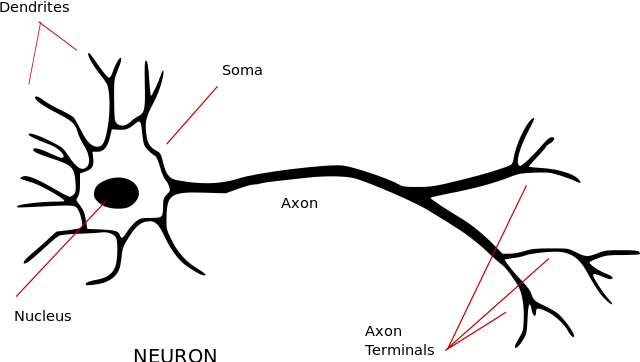
\includegraphics[width=8cm]{neuron.png}
  \end{center}
}
\caption{\textbf{A diagram of a neuron}; this cartoon shows the main parts of the neuron, very very roughly, the dendrites, where the signals come in, the soma where they get added together and the axon, which carries signals on to other neurons. Figure from \texttt{wikimedia}\label{fig_neuron}}
\end{figure}

There are two sorts of tubes extending from the soma, the
\textsl{dendrites} and the \textsl{axon}. These really are tubes,
though it is tempting to think of them as wires: the neuron has an
inside and an outside separated by a membrane. Both inside and outside
the neuron there is fluid, basically water with dissolved salts, but
the fluid inside and out have different concentrations of the ions
that make up the salts. There can be a potential difference, that is a
voltage difference, across the membrane and, as we will discuss, the
signals we are will be talking about are changes in voltage.

Roughly speaking, and this is a very rough claim, the signals to the
neuron come in along the dendrite whereas the signals the neuron sends
go out along the axon. The axon of other neurons will transmit signals
to this neuron's dendrites at points where they, the other neuron's
axon and this neuron's dendrite, nearly touch: the nearly-touching
place is called a synapses and synapses contains complicated
bio-mechanical machinery to allow the signals to be communicated from
axon to dendrite. We will discuss this further soon.

\begin{figure}[tbhp]
\ifthenelse{\boolean{nopics}}
{\textsl{A dark yellow picture has some neurons in a darker, browner colour, these are vaguely triangular shaped with thick lines running from them, largely up from their apex, other lines run in all directions from their base.}}
{
  \begin{center}
  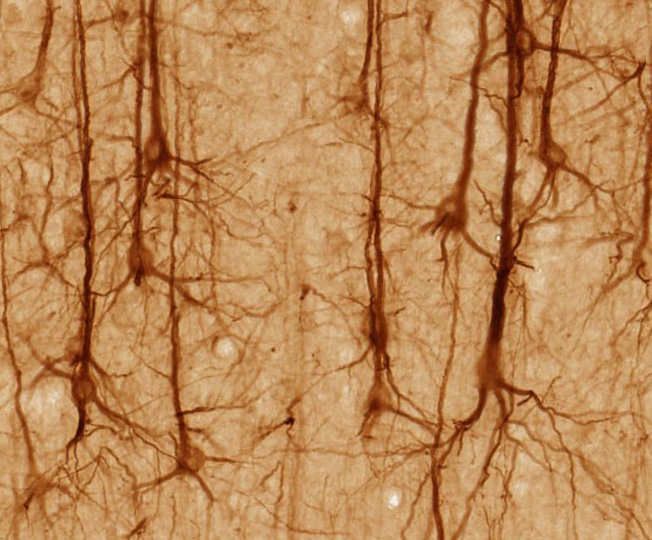
\includegraphics[width=6cm]{Smi32neuron.jpg}
  \end{center}
  }
  \caption{\textbf{A picture of some neurons}; these show the
    pyramidal neurons found in the cortex, part of the brain; they are
    called pyramidal because of the shape of the soma; you can also see the large number of dendrites. Figure from
    \texttt{wikipedia}\label{fig_real_neuron}}
\end{figure}

In Fig.~\ref{fig_real_neuron} is a picture of some neurons; it would
be a mistake to think that all neurons are similar to each
other. There is a huge diversity of different neurons, they differ in
their shape, in their size, in how connected they are and in their
voltage dynamics. As an extreme example, the Purkinje cells, as in
Fig.~\ref{fig_PC} has a huge number of dendrites and receives
connections from as many as 100\_000 other neurons, however, many of
those other neurons are cerebellum granule cells, very small neurons
that receive inputs from only three or four other neurons. 

\begin{figure}[tbhp]
\ifthenelse{\boolean{nopics}}
{\textsl{A line drawing showing a square maze of dense tiny lines, at its base is a black blob with a thicker line running downwards from it.}}
{
  \begin{center}
  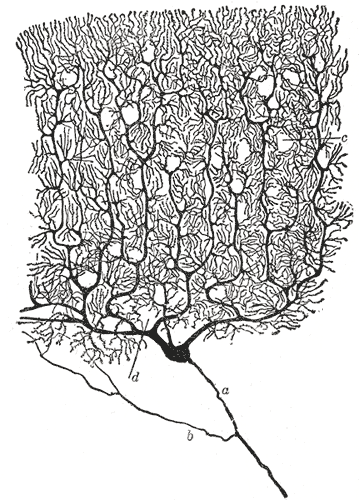
\includegraphics[width=5cm]{PC.png}
  \end{center}
  }
  \caption{\textbf{Drawing of a Purkinje cell}; this is a drawing of a
    Purkinje cell, by Santiago Ram\'{o}n y Cajal, an important
    neuroanatomist active in the late nineteenth and early twentieth
    century. The Purkinje cells are found in the cerebellum. Figure from
    \texttt{wikipedia}\label{fig_PC}}
\end{figure}

It is tempting, as a computer scientist, to think of neurons as a sort
of universal circuit component; this is a mistake. However, there are,
nonetheless, aspect to the description of neurons that are reasonably
general.The first of these reasonably general aspects we have already
covered: signals come in the dendrites, accumulate in the soma and go
out the axon. There is a more general aspect we have already alluded
to: the signals correspond to changes in voltage.

\subsection*{Action potentials}

There is a potential difference between the inside and outside of a
neuron. For convenience we usually regard the fluid in the brain as
being at a zero voltage; relative to that the fluid inside a neuron
has a negative voltage; -70 mV at rest would be a typical value. You
might think this makes no sense, if there is a voltage difference
between the inside and outside of the neuron, surely a current would
flow between the two equalizing the voltage difference? There are a
number of reasons that doesn't happen, firstly the membrane is an
insulator, largely preventing the flow of current, secondly, the
situation is, as we will see, more subtle, not only is there a
difference in voltage across the membrane, there is a difference in
the concentration of ions with, for example, an excess of sodium ions
outside the cell relative to inside and an excess of potassium ions
inside relative to out. Along with the voltage differences, these
concentration differences also have the potential to cause ions to
flow into or out of the neuron. Finally, there are pumps, minuscule
molecular machines, which pump ions in and out of the neuron to help
maintain the voltage difference. It is, all-in-all, a complicated
story, for now, what we need to know is that there is a voltage
difference across the cell membrane.

Why is this important: well it is important because the signaling
dynamics of a neuron is voltage dynamics: signals are carried by what
are called \textsl{action potentials} or \textsl{spikes}: these are
spikes in the voltage that travel along the axon. A picture of an
action potential is shown in Fig.~\ref{fig_hh}. During a spike the
voltage shoots up by about 80 mV and then falls back to near the
resting value, all during 1-2 ms. The dynamics that allow this to
happen come from ions traveling through the membrane, in a sense the
energy for the spike has been stored up by the all ion pumping that
has created the concentration differences across the membrane. The
spike will travel along the axon. The axon will usually have many
branches and when this happens a spike will travel down each branch:
the spike doesn't split in the sense that the spike traveling down
each branch will be the same size as the original spike. Similarly,
broadly speaking, the spike does not change amplitude or shape as it
propagates along the axon. I think a useful analogy here is to a train
of dominoes fall over; the energy in that case comes from the energy
stored in the domino when it was set upright, the collision from the
other domino hitting it is what causes it to fall over but isn't the
source of most of the energy involved in its own fall; when a train of
dominoes splits, the wave of falling-over is just as fast along each
branch.


\begin{figure}[tbhp]
\ifthenelse{\boolean{nopics}}
{\textsl{This looks like an old hand drawn graph, the curve is first horizontal, it suddenly rises upwards, has a roundish peak and then falls to a lower point than when it started, it resembles the first climb and fall of a rollercoaster in shope. After the fall is gradually rises to the level it started at.}}
{
  \begin{center}
  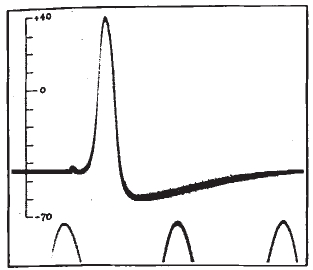
\includegraphics[width=6cm]{action_potential.jpg}
  \end{center}
  }
  \caption{\textbf{An action potential}; this is an action potential
    recorded from an axon, it is actually a very early recording
    performed by Hodgkin and Huxley, pioneers in recording and
    modeling action potentials; this picture is actually a photograph
    of an oscilloscope trace. \label{fig_hh}}
\end{figure}

\section{Summary}

So far we have begun a broad overview of neurons and what they do;
this is all going to be revisited in more detail later. In particular
we have described the division of neurons into dendrites, soma and
axons and have seen that signals propagate along the axon in the form
of voltage spikes.

\end{document}

